\documentclass[8pt,aspectratio=169]{beamer}
\usetheme{Madrid}
\usepackage{graphicx}
\usepackage{booktabs}
\usepackage{adjustbox}
\usepackage{multicol}
\usepackage{amsmath}
\usepackage{amssymb}
\usepackage{tikz}
\usetikzlibrary{arrows.meta,positioning,shapes.callouts,shapes.geometric,decorations.pathreplacing}
\usepackage{colortbl}
\usepackage{pgfplots}
\pgfplotsset{compat=1.18}
\usepackage{hyperref}
\usepackage{algorithm}
\usepackage{algorithmic}

% Color definitions
\definecolor{mlblue}{RGB}{0,102,204}
\definecolor{mlpurple}{RGB}{51,51,178}
\definecolor{mllavender}{RGB}{173,173,224}
\definecolor{mllavender2}{RGB}{193,193,232}
\definecolor{mllavender3}{RGB}{204,204,235}
\definecolor{mllavender4}{RGB}{214,214,239}
\definecolor{mlorange}{RGB}{255, 127, 14}
\definecolor{mlgreen}{RGB}{44, 160, 44}
\definecolor{mlred}{RGB}{214, 39, 40}
\definecolor{mlgray}{RGB}{127, 127, 127}

% Additional colors for template compatibility
\definecolor{lightgray}{RGB}{240, 240, 240}
\definecolor{midgray}{RGB}{180, 180, 180}
\definecolor{dfteal}{RGB}{0,128,128}
\definecolor{dfred}{RGB}{180,30,30}

% Backward compatibility: uppercase color names
\colorlet{MLPurple}{mlpurple}
\colorlet{MLBlue}{mlblue}
\colorlet{MLOrange}{mlorange}
\colorlet{MLGreen}{mlgreen}
\colorlet{MLRed}{mlred}
\colorlet{MLLavender}{mllavender}
\colorlet{MLGray}{mlgray}

% Apply custom colors to Madrid theme
\setbeamercolor{palette primary}{bg=mllavender3,fg=mlpurple}
\setbeamercolor{palette secondary}{bg=mllavender2,fg=mlpurple}
\setbeamercolor{palette tertiary}{bg=mllavender,fg=white}
\setbeamercolor{palette quaternary}{bg=mlpurple,fg=white}

\setbeamercolor{structure}{fg=mlpurple}
\setbeamercolor{section in toc}{fg=mlpurple}
\setbeamercolor{subsection in toc}{fg=mlblue}
\setbeamercolor{title}{fg=mlpurple}
\setbeamercolor{frametitle}{fg=mlpurple,bg=mllavender3}
\setbeamercolor{block title}{bg=mllavender2,fg=mlpurple}
\setbeamercolor{block body}{bg=mllavender4,fg=black}

% Remove navigation symbols
\setbeamertemplate{navigation symbols}{}

% Clean itemize/enumerate
\setbeamertemplate{itemize items}[circle]
\setbeamertemplate{enumerate items}[default]

% Reduce margins for more content space
\setbeamersize{text margin left=5mm,text margin right=5mm}

% Custom course footer
\setbeamertemplate{footline}{
  \leavevmode%
  \hbox{%
    \begin{beamercolorbox}[wd=.333333\paperwidth,ht=2.25ex,dp=1ex,center]{author in head/foot}%
      \usebeamerfont{author in head/foot}Methods and Algorithms
    \end{beamercolorbox}%
    \begin{beamercolorbox}[wd=.333333\paperwidth,ht=2.25ex,dp=1ex,center]{title in head/foot}%
      \usebeamerfont{title in head/foot}MSc Data Science
    \end{beamercolorbox}%
    \begin{beamercolorbox}[wd=.333333\paperwidth,ht=2.25ex,dp=1ex,right]{date in head/foot}%
      \usebeamerfont{date in head/foot}\insertframenumber{} / \inserttotalframenumber\hspace*{2ex}
    \end{beamercolorbox}}%
  \vskip0pt%
}

% Command for bottom annotation (Madrid-style)
\newcommand{\bottomnote}[1]{%
\vfill
\vspace{-2mm}
\textcolor{mllavender2}{\rule{\textwidth}{0.4pt}}
\vspace{1mm}
\footnotesize
\textbf{#1}
}

% Custom commands for course compatibility
\newcommand{\highlight}[1]{\textcolor{mlorange}{\textbf{#1}}}
\newcommand{\mathbold}[1]{\boldsymbol{#1}}

% Compact list environment
\newenvironment{compactlist}{%
  \begin{itemize}%
    \setlength{\itemsep}{2pt}%
    \setlength{\parskip}{0pt}%
    \setlength{\parsep}{0pt}%
}{%
  \end{itemize}%
}

\title[L06: Embeddings \& RL]{Embeddings \& RL: A Visual Guide}
\subtitle{Teaching Computers to Understand and Decide}
\author{Prof.\ Dr.\ J\"org Osterrieder}
\institute{Methods and Algorithms --- MSc Data Science}
\date{Spring 2026}

\begin{document}

%% ===== FRONT MATTER (3 slides) =====

% Slide 1: Title Page
\begin{frame}[plain]
\titlepage
\end{frame}

% Slide 2: XKCD Opening
\begin{frame}{How Do You Teach a Computer?}
\begin{columns}[c]
\begin{column}{0.45\textwidth}
\centering
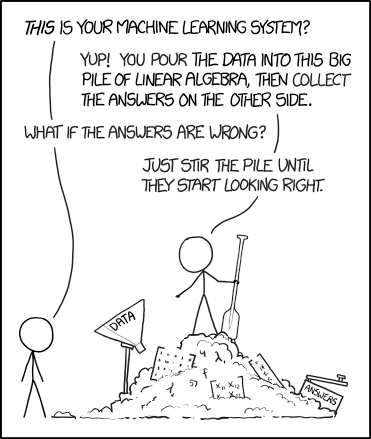
\includegraphics[height=0.55\textheight]{images/1838_machine_learning.png}
\end{column}
\begin{column}{0.50\textwidth}
\large
\textit{How do you teach a computer to \textbf{understand language} and \textbf{make decisions}?}

\vspace{6mm}
Today we explore two big ideas:
\begin{compactlist}
\item \textbf{Embeddings} --- understanding words
\item \textbf{RL} --- learning to act
\end{compactlist}
\end{column}
\end{columns}
\bottomnote{XKCD \#1838 by Randall Munroe (CC BY-NC 2.5)}
\end{frame}

% Slide 3: Learning Objectives
\begin{frame}{What You Will Learn Today}
\begin{enumerate}
\setlength{\itemsep}{8pt}
\item \textbf{Explain what word embeddings do} --- in plain English
\item \textbf{Describe how an RL agent learns} from rewards
\item \textbf{Choose when to use embeddings vs RL} for a problem
\end{enumerate}
\bottomnote{Everything is explained with pictures and analogies.}
\end{frame}

%% ===== ACT 1: THE PROBLEM (3 slides) =====

% Slide 4: TikZ Comic C1 --- "Lost in Translation"
\begin{frame}{The Problem: Computers Don't Understand Words!}
\centering
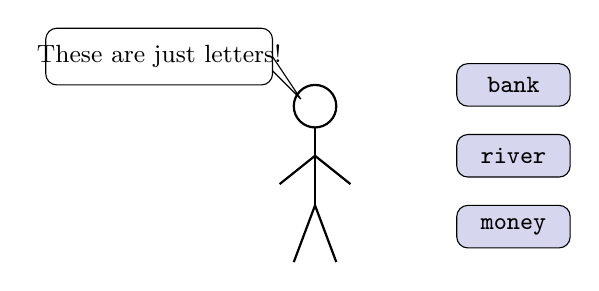
\begin{tikzpicture}[scale=0.9]
% Stick figure
\draw[thick] (0,2.2) circle (0.3);
\draw[thick] (0,1.9) -- (0,0.8);
\draw[thick] (0,1.5) -- (-0.5,1.1);
\draw[thick] (0,1.5) -- (0.5,1.1);
\draw[thick] (0,0.8) -- (-0.3,0);
\draw[thick] (0,0.8) -- (0.3,0);
% Word cards
\draw[fill=mllavender4, rounded corners] (2.0,2.2) rectangle (3.6,2.8);
\node at (2.8,2.5) {\small\texttt{bank}};
\draw[fill=mllavender4, rounded corners] (2.0,1.2) rectangle (3.6,1.8);
\node at (2.8,1.5) {\small\texttt{river}};
\draw[fill=mllavender4, rounded corners] (2.0,0.2) rectangle (3.6,0.8);
\node at (2.8,0.5) {\small\texttt{money}};
% Speech bubble
\draw[fill=white, rounded corners] (-3.8,2.5) rectangle (-0.6,3.3);
\draw (-0.6,2.7) -- (-0.2,2.3) -- (-0.6,2.9);
\node at (-2.2,2.9) {\small These are just letters!};
\end{tikzpicture}

\vspace{2mm}
A computer sees text as a string of characters. It has no concept of meaning.
\bottomnote{Computers need numbers, not words. But which numbers capture meaning?}
\end{frame}

% Slide 5: CHART --- Word Embedding Space
\begin{frame}{Words Can Become Points in Space!}
\centering

\includegraphics[width=0.65\textwidth]{01_word_embedding_space/chart.pdf}
\begin{compactlist}
\item Each word is placed at a specific location (coordinates)
\item Similar words end up close together
\item The computer learned these positions from reading text
\end{compactlist}
\bottomnote{Word embeddings turn words into vectors --- lists of numbers that capture meaning.}
\end{frame}

% Slide 6: Why Can't We Just Number Words 1, 2, 3?
\begin{frame}{Why Not Just Number Every Word?}
\begin{columns}[T]
\begin{column}{0.47\textwidth}
\textcolor{mlred}{\textbf{Simple Numbering}}
\begin{compactlist}
\item cat = 1, dog = 2, car = 3
\item dog is NOT ``between'' cat and car
\item Numbers imply an order that doesn't exist
\end{compactlist}
\end{column}
\begin{column}{0.47\textwidth}
\textcolor{mlgreen}{\textbf{Embeddings}}
\begin{compactlist}
\item cat = [0.9, 0.1]
\item dog = [0.8, 0.2]
\item car = [0.1, 0.7]
\end{compactlist}
\vspace{2mm}
cat and dog are close (both animals). car is far away (different concept).
\end{column}
\end{columns}
\vspace{3mm}
\begin{block}{Key Insight}
Embeddings capture relationships. Simple numbers don't.
\end{block}
\bottomnote{Embeddings are learned from data --- the computer discovers which words are similar by seeing them in context.}
\end{frame}

%% ===== ACT 2: EMBEDDINGS = ADDRESSES FOR WORDS (6 slides) =====

% Slide 7: TikZ Comic C2 --- "Words as Addresses"
\begin{frame}{Embeddings = Giving Words a Home Address}
\centering
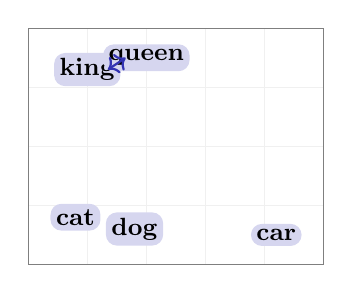
\begin{tikzpicture}[scale=0.75]
% Grid
\draw[step=1, lightgray, thin] (0,0) grid (5,4);
\draw[mlgray] (0,0) rectangle (5,4);
% Word labels at positions
\node[fill=mllavender4, rounded corners, inner sep=2pt] at (1.0,3.3) {\small\textbf{king}};
\node[fill=mllavender4, rounded corners, inner sep=2pt] at (2.0,3.5) {\small\textbf{queen}};
\draw[<->, mlpurple, thick] (1.35,3.3) -- (1.65,3.5);
\node[fill=mllavender4, rounded corners, inner sep=2pt] at (0.8,0.8) {\small\textbf{cat}};
\node[fill=mllavender4, rounded corners, inner sep=2pt] at (1.8,0.6) {\small\textbf{dog}};
\node[fill=mllavender4, rounded corners, inner sep=2pt] at (4.2,0.5) {\small\textbf{car}};
\end{tikzpicture}

\vspace{2mm}
Similar words live in the same neighborhood.
\bottomnote{In a city, nearby addresses mean nearby locations. In embeddings, nearby vectors mean similar meanings.}
\end{frame}

% Slide 8: CHART --- Word Analogy
\begin{frame}{The Magic of Word Math!}
\centering

\includegraphics[width=0.60\textwidth]{top10_08_word_analogy/chart.pdf}
\begin{compactlist}
\item King $-$ Man $+$ Woman $=$ Queen
\item Paris $-$ France $+$ Germany $=$ Berlin
\item Embeddings capture analogies as vector arithmetic
\end{compactlist}
\bottomnote{This is the ``aha moment'' of embeddings: meaning has direction. Gender, country, tense --- all are vectors.}
\end{frame}

% Slide 9: How Are Embeddings Made? (TikZ flowchart)
\begin{frame}{How Embeddings Are Made}
\centering
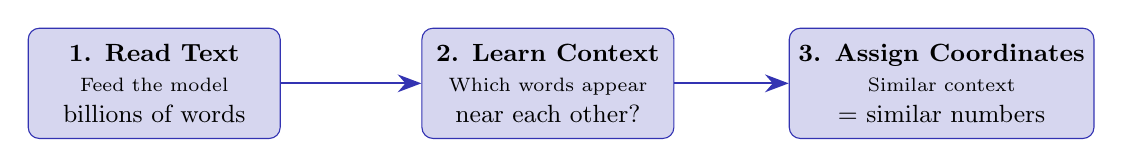
\begin{tikzpicture}[
  box/.style={draw=mlpurple, fill=mllavender4, rounded corners, minimum width=3.2cm, minimum height=1.4cm, align=center, font=\small},
  arr/.style={-{Stealth[length=3mm]}, thick, mlpurple}
]
\node[box] (a) at (0,0) {\textbf{1. Read Text}\\\scriptsize Feed the model\\billions of words};
\node[box] (b) at (5,0) {\textbf{2. Learn Context}\\\scriptsize Which words appear\\near each other?};
\node[box] (c) at (10,0) {\textbf{3. Assign Coordinates}\\\scriptsize Similar context\\= similar numbers};
\draw[arr] (a) -- (b);
\draw[arr] (b) -- (c);
\end{tikzpicture}

\vspace{5mm}
That's it. The computer reads text and figures out which words are similar.
\bottomnote{Word2Vec, GloVe, and BERT all follow this principle: learn from context.}
\end{frame}

% Slide 10: CHART --- Similarity Heatmap
\begin{frame}{Who Is Similar to Whom?}
\centering

\includegraphics[width=0.60\textwidth]{02_similarity_heatmap/chart.pdf}
\begin{compactlist}
\item Dark squares = highly similar words
\item Light squares = unrelated words
\item The computer learned this from reading text alone --- no human labeled it
\end{compactlist}
\bottomnote{Cosine similarity measures the angle between two word vectors. Small angle = similar meaning.}
\end{frame}

% Slide 11: Finance Application
\begin{frame}{Why Bankers Care About Embeddings}
\begin{compactlist}
\item \textbf{Sentiment Analysis}: Is this news article positive or negative for the stock?
\item \textbf{Fraud Detection}: Does this transaction description look suspicious?
\item \textbf{Document Search}: Find contracts similar to this one
\end{compactlist}
\vspace{3mm}
\begin{block}{Bottom Line}
Embeddings let machines understand financial text --- reports, news, filings.
\end{block}
\bottomnote{JPMorgan, Goldman Sachs, and Bloomberg all use NLP with embeddings for financial analysis.}
\end{frame}

% Slide 12: Transition
\begin{frame}{Understanding Is Powerful, But What About Action?}
\centering
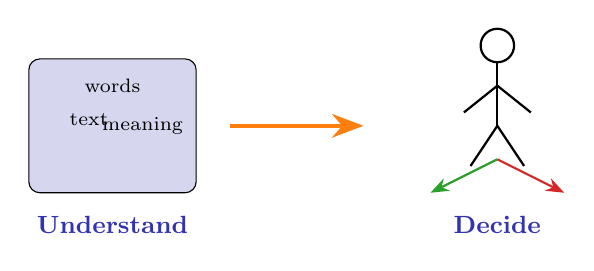
\begin{tikzpicture}[scale=0.85]
% Left: word bubble
\draw[fill=mllavender4, rounded corners] (-3.5,-0.5) rectangle (-1.0,1.5);
\node[font=\scriptsize] at (-2.25,1.1) {words};
\node[font=\scriptsize] at (-2.6,0.6) {text};
\node[font=\scriptsize] at (-1.8,0.5) {meaning};
\node[font=\small, mlpurple, below] at (-2.25,-0.7) {\textbf{Understand}};
% Arrow
\draw[-{Stealth[length=4mm]}, ultra thick, mlorange] (-.5,0.5) -- (1.5,0.5);
% Right: stick figure at crossroads
\draw[thick] (3.5,1.7) circle (0.25);
\draw[thick] (3.5,1.45) -- (3.5,0.5);
\draw[thick] (3.5,1.1) -- (3.0,0.7);
\draw[thick] (3.5,1.1) -- (4.0,0.7);
\draw[thick] (3.5,0.5) -- (3.1,-0.1);
\draw[thick] (3.5,0.5) -- (3.9,-0.1);
\draw[-{Stealth}, thick, mlgreen] (3.5,0.0) -- (2.5,-0.5);
\draw[-{Stealth}, thick, mlred] (3.5,0.0) -- (4.5,-0.5);
\node[font=\small, mlpurple, below] at (3.5,-0.7) {\textbf{Decide}};
\end{tikzpicture}

\vspace{2mm}
\begin{compactlist}
\item Embeddings teach computers to \textbf{understand} language
\item But some problems require making \textbf{sequential decisions} under uncertainty
\end{compactlist}
\bottomnote{Embeddings answer ``what does this mean?'' RL answers ``what should I do next?''}
\end{frame}

%% ===== ACT 3: RL = LEARNING BY DOING (7 slides) =====

% Slide 13: TikZ Comic C3 --- "The Maze Runner"
\begin{frame}{RL: Learning by Trying, Failing, and Trying Again}
\centering
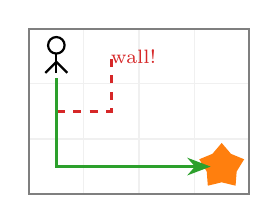
\begin{tikzpicture}[scale=0.7]
% Grid (maze)
\draw[step=1, lightgray] (0,0) grid (4,3);
\draw[mlgray, thick] (0,0) rectangle (4,3);
% Stick figure at start
\draw[thick] (0.5,2.7) circle (0.15);
\draw[thick] (0.5,2.55) -- (0.5,2.2);
\draw[thick] (0.5,2.4) -- (0.3,2.2);
\draw[thick] (0.5,2.4) -- (0.7,2.2);
% Star at goal
\node[star, star points=5, fill=mlorange, minimum size=6mm] at (3.5,0.5) {};
% Wrong path (dashed)
\draw[dashed, mlred, thick] (0.5,2.1) -- (0.5,1.5) -- (1.5,1.5) -- (1.5,2.5);
\node[font=\scriptsize, mlred] at (1.9,2.5) {wall!};
% Learned path (solid)
\draw[mlgreen, very thick, -{Stealth}] (0.5,2.1) -- (0.5,0.5) -- (3.3,0.5);
\end{tikzpicture}

\vspace{2mm}
The agent doesn't know the map --- it learns by exploring.
\bottomnote{Reinforcement Learning = learn from experience, not from labeled examples.}
\end{frame}

% Slide 14: CHART --- The RL Loop
\begin{frame}{The Core Idea: Act, Observe, Learn, Repeat}
\centering

\includegraphics[width=0.55\textwidth]{03_rl_loop/chart.pdf}
\vspace{-1mm}
\begin{compactlist}
\item The agent takes an action in the environment
\item The environment gives back a reward (or penalty)
\item The agent updates its strategy and tries again
\end{compactlist}
\bottomnote{This loop is the foundation of ALL reinforcement learning. Everything else is optimization.}
\end{frame}

% Slide 15: CHART --- Q-Learning Grid
\begin{frame}{Watch the Agent Learn the Best Path}
\centering

\includegraphics[width=0.55\textwidth]{04_q_learning_grid/chart.pdf}
\vspace{-2mm}
\begin{compactlist}
\item Arrows show the agent's best guess for direction
\item After many episodes, arrows converge to the optimal path
\item Discovered by trial and error --- no teacher told it
\end{compactlist}
\bottomnote{Q-learning stores a ``quality'' score for each state-action pair. Higher Q = better action.}
\end{frame}

% Slide 16: How RL Works (No Math)
\begin{frame}{How RL Works (No Math)}
\begin{enumerate}
\setlength{\itemsep}{5pt}
\item \textbf{Try an action} --- the agent does something (move left, buy, sell)

\begin{tikzpicture}[baseline=-0.5ex]
\draw[-{Stealth}, thick, mlblue] (0,0) -- (0.7,0);
\end{tikzpicture}
\item \textbf{Get feedback} --- the environment gives a reward (+1) or penalty ($-$1)

\begin{tikzpicture}[baseline=-0.5ex]
\node[star, star points=5, fill=mlorange, minimum size=4mm] at (0,0) {};
\end{tikzpicture}
\item \textbf{Update strategy} --- remember what worked, avoid what didn't

\begin{tikzpicture}[baseline=-0.5ex]
\draw[thick, mlpurple] (0,0) circle (0.2);
\draw[thick, mlpurple] (-0.15,0.25) -- (-0.05,0.4);
\draw[thick, mlpurple] (0.15,0.25) -- (0.05,0.4);
\draw[thick, mlpurple] (0,0.25) -- (0,0.4);
\end{tikzpicture}
\end{enumerate}
\vspace{3mm}
\begin{block}{The Secret}
Repeat thousands of times. The agent gets better.
\end{block}
\bottomnote{RL agents typically need millions of episodes to learn. That is why simulation is so important.}
\end{frame}

% Slide 17: CHART --- Reward Curves
\begin{frame}{Proof It Works: Rewards Go Up Over Time}
\centering

\includegraphics[width=0.60\textwidth]{05_reward_curves/chart.pdf}
\begin{compactlist}
\item The y-axis shows cumulative reward
\item The line goes up = the agent is getting better
\item Early episodes are random; later episodes show learned behavior
\end{compactlist}
\bottomnote{A rising reward curve is the universal sign of a learning agent. Flat = stuck. Dropping = broken reward.}
\end{frame}

% Slide 18: CHART --- Explore vs Exploit
\begin{frame}{The Key Tradeoff: Explore or Exploit?}
\centering

\includegraphics[width=0.60\textwidth]{top10_09_epsilon_greedy/chart.pdf}
\begin{compactlist}
\item \textbf{Explore} = try something new (might find better)
\item \textbf{Exploit} = stick with what works (safe but might miss better)
\item Epsilon-greedy: explore with probability epsilon, exploit otherwise
\end{compactlist}
\bottomnote{Too much exploration = never settles. Too much exploitation = misses the best strategy.}
\end{frame}

% Slide 19: RL Gotchas
\begin{frame}{Three Things to Watch Out For}
\begin{enumerate}
\setlength{\itemsep}{6pt}
\item \textcolor{mlred}{\textbf{!}} \textbf{Needs LOTS of practice} --- millions of episodes. That's why we train in simulation first.
\item \textcolor{mlred}{\textbf{!}} \textbf{Reward design is tricky} --- the agent finds loopholes you didn't expect. Design rewards carefully.
\item \textcolor{mlred}{\textbf{!}} \textbf{Sim-to-real gap} --- what works in simulation may not work in the real world without fine-tuning.
\end{enumerate}
\bottomnote{RL is powerful but hungry: it needs massive compute and careful reward engineering.}
\end{frame}

%% ===== ACT 4: WHEN TO USE WHAT (4 slides) =====

% Slide 20: Embeddings vs RL Side-by-Side
\begin{frame}{Embeddings vs RL: Quick Comparison}
\centering
\small
\begin{tabular}{l c c}
\toprule
\textbf{Aspect} & \textbf{Embeddings} & \textbf{RL} \\
\midrule
Input & Text / documents & Actions / states \\
Output & Number representations & Decisions / policies \\
Learns from & Patterns in text & Rewards and penalties \\
Speed & Fast (minutes) & Slow (hours to days) \\
Use case & Understanding & Acting \\
\bottomrule
\end{tabular}

\vspace{4mm}
\highlight{They solve different problems. Use embeddings to understand, RL to act.}
\bottomnote{In practice, you can combine them: embeddings as state representation for RL agents.}
\end{frame}

% Slide 21: CHART --- Decision Flowchart
\begin{frame}{Which Method Should I Use?}
\centering

\includegraphics[width=0.55\textwidth]{07_decision_flowchart/chart.pdf}
\vspace{-2mm}
\begin{compactlist}
\item Start at the top and follow the arrows
\item In practice, many real systems combine both
\end{compactlist}
\bottomnote{When in doubt: embeddings for text understanding, RL for sequential decision-making.}
\end{frame}

% Slide 22: Finance Teaser
\begin{frame}{AI in Finance: Embeddings + RL}
\begin{columns}[T]
\begin{column}{0.47\textwidth}
\textcolor{mlpurple}{\textbf{Embeddings in Finance}}
\begin{compactlist}
\item Chatbots for customer service
\item Credit scoring from application text
\item ESG report analysis at scale
\end{compactlist}
\end{column}
\begin{column}{0.47\textwidth}
\textcolor{mlblue}{\textbf{RL in Finance}}
\begin{compactlist}
\item Algorithmic trading strategies
\item Portfolio rebalancing
\item Optimal order execution
\end{compactlist}
\end{column}
\end{columns}
\bottomnote{The biggest banks and hedge funds use both: NLP for understanding markets, RL for acting on them.}
\end{frame}

% Slide 23: The Python Recipe
\begin{frame}{Try It Yourself}
\begin{columns}[T]
\begin{column}{0.47\textwidth}
\textcolor{mlpurple}{\textbf{Embeddings (3 lines)}}

\vspace{2mm}
\footnotesize
\texttt{from gensim.models import Word2Vec}\\[1pt]
\texttt{model = Word2Vec(sentences,}\\
\texttt{~~~~~~~~~~~~~~~~vector\_size=100)}\\[1pt]
\texttt{similar = model.wv.most\_similar("bank")}
\end{column}
\begin{column}{0.47\textwidth}
\textcolor{mlblue}{\textbf{RL (plain English)}}

\vspace{2mm}
\footnotesize
\texttt{for each episode:}\\[1pt]
\texttt{~~observe state, pick action}\\[1pt]
\texttt{~~get reward, update strategy}\\[1pt]
\texttt{~~repeat until done}
\end{column}
\end{columns}
\vspace{4mm}
\small Embeddings: 3 lines of real Python. RL: the algorithm in plain English.
\bottomnote{For embeddings: pip install gensim. For RL: start with OpenAI Gym environments.}
\end{frame}

%% ===== CLOSING (3 slides) =====

% Slide 24: TikZ Comic C4 --- "Now the Computer Understands"
\begin{frame}{From Confusion to Intelligence}
\centering
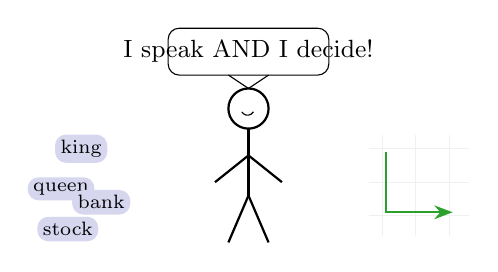
\begin{tikzpicture}[scale=0.85]
% Word cluster (left)
\node[fill=mllavender4, rounded corners, inner sep=2pt, font=\scriptsize] at (-2.5,1.0) {king};
\node[fill=mllavender4, rounded corners, inner sep=2pt, font=\scriptsize] at (-2.8,0.4) {queen};
\node[fill=mllavender4, rounded corners, inner sep=2pt, font=\scriptsize] at (-2.2,0.2) {bank};
\node[fill=mllavender4, rounded corners, inner sep=2pt, font=\scriptsize] at (-2.7,-0.2) {stock};
% Stick figure (center, happy)
\draw[thick] (0,1.6) circle (0.3);
\draw (-.1,1.55) arc (210:330:0.1); % smile
\draw[thick] (0,1.3) -- (0,0.3);
\draw[thick] (0,0.9) -- (-0.5,0.5);
\draw[thick] (0,0.9) -- (0.5,0.5);
\draw[thick] (0,0.3) -- (-0.3,-0.4);
\draw[thick] (0,0.3) -- (0.3,-0.4);
% Speech bubble
\draw[fill=white, rounded corners] (-1.2,2.1) rectangle (1.2,2.8);
\draw (-0.3,2.1) -- (0,1.9) -- (0.3,2.1);
\node[font=\small] at (0,2.45) {I speak AND I decide!};
% Grid with path (right)
\draw[step=0.5, lightgray, thin] (1.8,-0.3) grid (3.3,1.2);
\draw[mlgreen, thick, -{Stealth}] (2.05,0.95) -- (2.05,0.05) -- (3.05,0.05);
\end{tikzpicture}

\vspace{2mm}
Embeddings teach understanding. RL teaches action. Together: modern AI.
\bottomnote{Embeddings teach understanding. RL teaches action. Together, they are the foundation of modern AI.}
\end{frame}

% Slide 25: Key Takeaways
\begin{frame}{Five Things to Remember}
\begin{enumerate}
\setlength{\itemsep}{5pt}
\item Embeddings turn words into numbers that capture meaning
\item Similar words get similar numbers --- the computer learns this from text
\item RL agents learn by trial and error with rewards
\item Explore vs exploit is the key RL tradeoff
\item Both are used in finance: embeddings for text, RL for decisions
\end{enumerate}
\bottomnote{Embeddings for understanding. RL for acting. Use both.}
\end{frame}

% Slide 26: XKCD Closing
\begin{frame}{Go Teach a Machine Something}
\centering
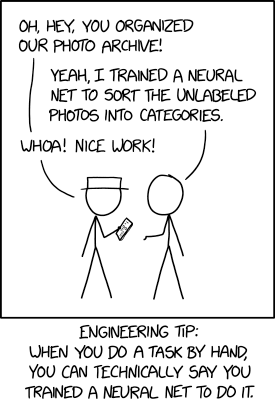
\includegraphics[height=0.55\textheight]{images/2173_trained_a_neural_net.png}
\bottomnote{XKCD \#2173 by Randall Munroe (CC BY-NC 2.5). Next: try the Jupyter notebook with real financial data!}
\end{frame}

\end{document}
